Salim et al.\cite{Salim2019} have presented a thorough survey of a number of different DDoS
attacks which are common in IoT networks. Their work provides classifications
for these attacks, along with providing a number of detection, prevention and
mitigation solutions.

\begin{figure}[H]
	\centering
	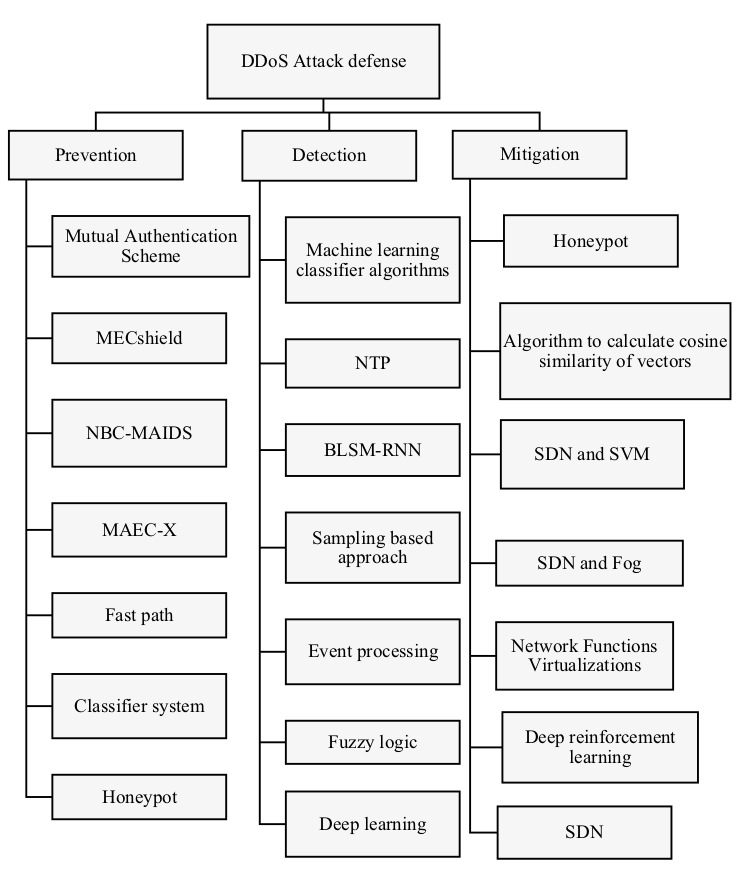
\includegraphics[width=0.5\textwidth]{images/salimDefenseDiagram.png}
	\caption{Salim et al. DDoS attack Defence techniques\cite{Salim2019}}
	\label{fig:salimDefense}
\end{figure}

As seen in Figure \ref{fig:salimDefense}, there are 21 proposed solutions; 7
Prevention, 7 Detection, and 7 Mitigation. These solutions act at the device
level, edge computing level, and cloud level.

Prevention of attacks deals in stopping traffic flow between nodes flagged for
suspicious or ``abnormal'' traffic. These techniques involve
monitoring the traffic between the nodes, and either stopping data flow (Mutual
Authentication Scheme), highlighting suspicious traffic to other nodes in the
network (MECshield, NBC-MAIDS, Multi-access Edge Computing, Fast Path,
Classifier System), or diverting attack traffic (Honeypot).

Detection of attacks deals in correctly detecting that the traffic flow is due
to an attack. These techniques utilise machine learning (Machine Learning
Classifier Algorithms, BLSM-RNN, Fuzzy Logic, Deep Learning) and event processing
(CEPID, Sampling-based Approach) in order to detect attack traffic, in some
cases, with very high accuracy. The Machine Learning Classifier Algorithms
technique had a recorded detection accuracy in real time IoT devices of 0.99\%.

Mitigation of attacks deals in stopping a detected DDoS attack. This attack
mitigation is implemented by blocking dataflow from malicious nodes within the
network (SDN and SVM, ECESID, Deep Reinforcement Learning, and SDN).
